% Created 2019-06-21 ven. 13:36
\documentclass{article}
\usepackage[utf8]{inputenc}
\usepackage[T1]{fontenc}
\usepackage{fixltx2e}
\usepackage{graphicx}
\usepackage{longtable}
\usepackage{float}
\usepackage{wrapfig}
\usepackage{rotating}
\usepackage[normalem]{ulem}
\usepackage{amsmath}
\usepackage{textcomp}
\usepackage{marvosym}
\usepackage{wasysym}
\usepackage{amssymb}
\usepackage{hyperref}
\tolerance=1000
\usepackage[frenchb]{babel}
\date{\today}
\title{TP3 : Une interface pour le PacMan}
\hypersetup{
  pdfkeywords={},
  pdfsubject={},
  pdfcreator={Emacs 25.2.2 (Org mode 8.2.10)}}
\begin{document}

\maketitle

\section{L'interface}
\label{sec-1}
Le design pattern Modèle-Vue-Contrôleur est un design pattern destiné aux interfaces utilisateur. Il permet de dissocier les différents composants d'une application et de pouvoir les développer séparément.


\noindent
Lors de ce TP, vous aurez à réaliser la vue \verb~PacManView~ associée à cet ensemble modèle/contrôleur:

\begin{center}
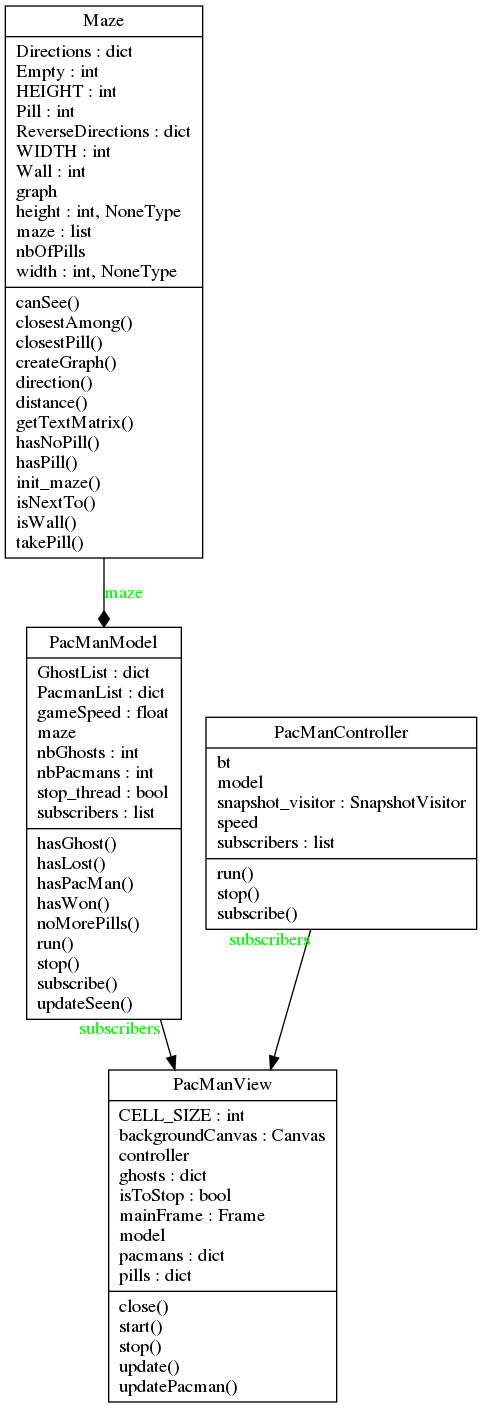
\includegraphics[width=0.25\linewidth]{./img/m_v_c.png}
\end{center}

\noindent
Le dernier exercice du TP précédent vous permet d'avoir les bases pour l'affichage du labyrinthe.
Maintenant il vous faut placer les PacGums, représentés par des 1 dans le tableau.

\noindent
Il faut bien faire attention de se rappeler des identifiants de ces PacGums, vous aurez à les supprimer lorsque le PacMan les mangera.
Le mieux pour cela est d'utiliser un dictionnaire avec leurs coordonnées comme clefs.

\noindent
Pour savoir s'il y a un PacGum à une coordonnée, n'oubliez pas d'utiliser \verb~model.maze.hasPill(x,y)~.

\noindent
La méthode \verb~updatePacman(p)~ permet de déplacer le Pacman et en même temps de l'orienter dans la bonne direction.
Cette méthode doit être appelée dans la méthode \verb~update()~.

\noindent
La méthode \verb~update()~ doit contenir la mise à jour des positions des Pacmans et des Fantômes, ainsi que la suppression des PacGums qui auraient été mangés.

\noindent
La construction du labyrinthe ainsi que le placement des PacGums doivent être réalisés dans la méthode \verb~start()~ qui doit elle-même être lancée à la fin de l'initialisation.

\noindent
Pour s'assurer de la bonne terminaison du programme, veuillez ajouter une ligne pemettant de changer la fonction à appeler en cas de fermeture de fenêtre ( \verb~fenetre.protocol("WM_DELETE_WINDOW",self.close)~), et faire en sorte que \verb~self.close()~ appelle la méthode \verb~stop()~ du contrôleur. 

Au final, votre fenêtre devra ressembler à ceci:

\begin{center}
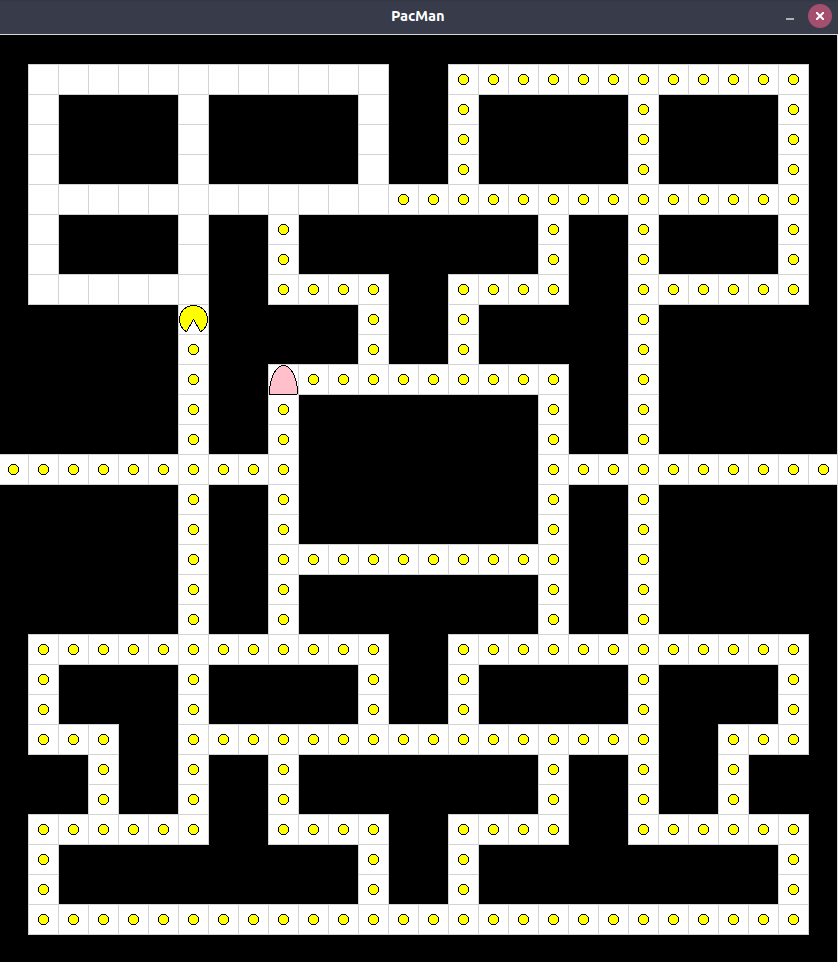
\includegraphics[width=.5\linewidth]{./img/PacMan.png}
\end{center}

\section{Le contrôleur (facultatif)}
\label{sec-2}

Si il vous reste du temps, vous pouvez jouer avec le contrôleur et modifier le comportement du PacMan ou du Fantôme.
% Emacs 25.2.2 (Org mode 8.2.10)
\end{document}